 
\section{The Schedule}

\subsection{Initial planning}

I divided the load of work of my project into four clear stages. The first one
was dedicated to study the feasability of the project and to do the initial
planning of the project. This was done through a course called \ac{GEP}. This
course includes the following stages:

\mylist
  \item Scope of the project.
  \item Project planning.
  \item Budget and sustainability.
  \item Preliminary presentation.
  \item Bibliography.
  \item List of conditions.
  \item Oral presentation and delivery of the final document.
\mylistend

\subsubsection*{Project analysis and design}

After taking the \ac{GEP} course, I moved on and started the stage of ``Project
analysis and design''. The main goal of this stage was to draw a clear picture
of the project and analyze all the goals of the project.

Therefore, this stage was made out of two sub stages. The first one, the
analysis of the project. In this sub stage I devoted myself to define all
the goals, requirements, features and use cases of my plaform. The other sub
stage consisted in design of the platform itself.

\subsubsection*{Project iterations}

\begin{enumerate}
\item {\bf Development of the core software infrastructure}

In this iteration I focused on the core infrastructure that has to
hold the whole platform. This was executed only in the software front.

\item {\bf Providing services}

The next iteration consisted on building the services on top of the base
infrastructure that had been created in the previous stage.

\item {\bf Designing the cluster}

At this point, we had the software ready to be deploy in production. So in this
step I focused on writing down the specifications of an ideal cluster.

\item {\bf Concluding the development}

In the last iteration I concluded the development of this project: running
tests, final checks of the code, etc.
\end{enumerate}


\subsubsection*{Final stage}

The final stage consisted on closing the project. The main points of this stage
were:

\mylist
  \item Write the documentation of the platform.
  \item Write the Final report (this document).
  \item Give the lecture of my thesis (June 27, 2014).
\mylistend

\subsubsection*{Gantt chart}

This initial planning was summarized in the following Gantt chart:

\begin{figure}[H]
  \hspace*{-2cm}
  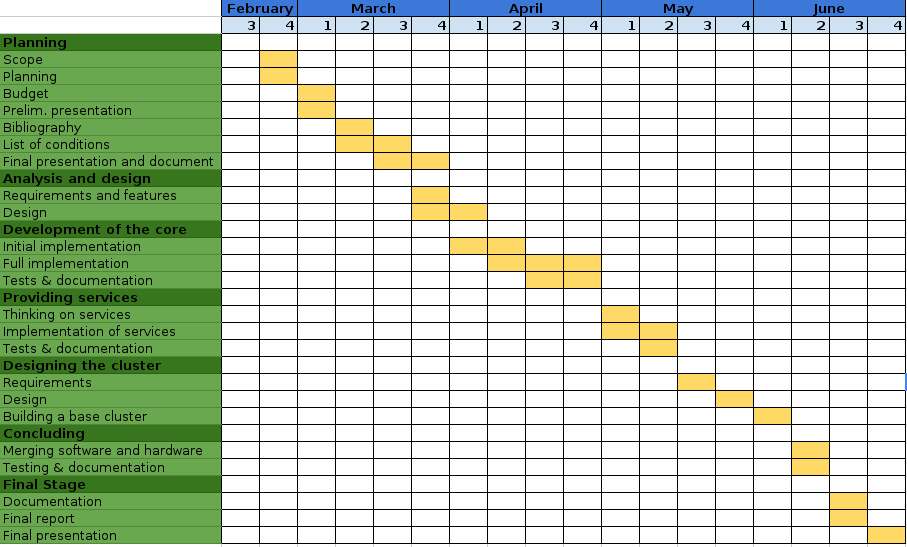
\includegraphics[scale=0.75]{development/images/gantt.png}
  \caption{Gantt chart}\label{fig:gantt}
\end{figure}

One thing to note is that I computed my work load in weeks instead of computing
it with hours. This might be odd, but it proved to be clear and simple. In my
final report of the \ac{GEP} course I stated that the total amount of hours per
day was not fixed. However, I changed this policy to a much saner approach:

\mylist
  \item On {\bf weekdays} I dedicated 2 hours per day. This is because I had a
day to day job and I also took more courses at university. This meant that I
could not spent too much time during weekdays. Approximately, though, I
dedicated 2 hours per day.
  \item On the {\bf weekend} I dedicated approximately 8 hours to this project.
\mylistend

As you can see, I have been quite flexible regarding hours dedicated per day.
Anyways, in total I have spent 17 weeks developing this project . This means
that in total I have spent approximately:

\begin{center}
  17 weeks $\times$ (5 weekdays $\times$ 2 hours + 8 hours on the
weekend) $=$ 306 hours
\end{center}

\subsection{Changes in the midterm evaluation}

There have not been any major change to my initial schedule. I have to admit
that for personal reasons I started the project a couple of weeks later
than expected. This means that by my midterm evaluation (``Fita de
seguiment''), my final schedule shifted a bit from my original one. This did not
result into many problems because:

\mylist
  \item In my orignal Gantt I kept the ``Analysis and design'' and the
``Development of the core'' phases seperately. I merged these two phases into
one. This turned out to be fine.
  \item The ``Providing services'' phase was shorter than expected.
\mylistend

\subsection{Final changes}

Apart from my changes on the schedule by the time of my midterm evaluation, I
did not have to do anymore changes in my schedule. The changes on the schedule
did not affect negatively in the development of this project.

\subsection{Conclusions}

As you have seen, my initial schedule was surprisingly on point. I only had to
do some minor changes on the schedule by the times of the midterm evaluation
and that was it.

Even though I followed the schedule successfully, during the development of
this project I felt that I was working too much during the stages ``Development
of the core'' and ``Providing services''. I think that one of the weakest
points of my initial schedule was that I decided to spend too much time on
stages like ``Planning'' and ``Analysis and design''. I probably could have
shortened this two stages, so I had more time on other stages that required
more hard work.
